\documentclass[pdftex,twocolumn,epjc3]{svjour3}          % twocolumn

\RequirePackage[T1]{fontenc}

\smartqed  % flush right qed marks, e.g. at end of proof

\usepackage{graphicx,amstext,amsmath,amsfonts,mathptmx,epstopdf,subfigure,float}
	
\RequirePackage[numbers,sort&compress]{natbib}
\RequirePackage[colorlinks,citecolor=blue,urlcolor=blue,linkcolor=blue]{hyperref}

%\journalname{Eur. Phys. J. C}

\begin{document}

\title{An approach to detect video frame deletion under anti-forensics\thanks{This work was supported in part by the National Key Research and Development of China (2018YFC0807306), National NSF of China (61672090, 61332012, 61532005), and Fundamental Research Funds for the Central Universities (2018JBZ001).}}


\author{Haichao Yao
\and
Rongrong Ni
\and
Yao Zhao}
\institute{Institute of Information Science, Beijing Jiaotong University, Beijing 100044, China
\and
Beijing Key Laboratory of Advanced Information Science and Network Technology, Beijing 100044, China}

\date{Received: date / Accepted: date}

\maketitle

\begin{abstract}
As a simple yet effective operation, frame deletion is widely
used in video forgery. Many video forensic techniques have been
developed to detect this manipulation. Some inter-frame
continuity based methods are capable to detect frame deletion as well as
locate the frame deletion points precisely. Due to the simple principle,
this kind of inter-frame continuity based methods are vulnerable to anti-forensic
strategies. In this paper, we first put forward an inter-frame interpolation method as anti-forensics which is very likely to occur. Then, to detect video frame deletion under anti-forensics, we analyse
the new artifacts introduced by interpolation, and present a global and local joint feature to distinguish the interpolated frames
and pristine frames. The feature overcomes the problem of weak residual in HEVC videos, and the low dimension ensures the real-time detection.
Experimental results show that the anti-forensic view we proposed needs to be considered in frame deletion forensics. And the proposed global and local joint feature can detect frame deletion under anti-forensic operation effectively.
\keywords{Video forensics \and frame deletion \and interpolated frames \and compression artifacts}
% \PACS{PACS code1 \and PACS code2 \and more}
% \subclass{MSC code1 \and MSC code2 \and more}
\end{abstract}

\section{Introduction}
\label{intro}
With the popularity of social applications, multimedia data such as images and videos are growing massively every minute. Owing to the development of some powerful editing tools, it is common for multimedia data to be maliciously modified. To cope with such problems, many digital forensic methods have been proposed in overviews \cite{A1,A2,A3}. As a simple way of video tampering, frame deletion can destroy significant information in a video without leaving visible traces. In this paper, we consider the forensics with respect to video frame deletion.

The forensic techniques towards frame deletion detection can be roughly divided into two categories.
The first category is based on the artifacts left by re-compression. In \cite{A4}, Wang and Farid found a periodical spikes on the motion residual histogram when the I-frame changed into P-frame because of frame deletion. In \cite{A5}, Luo \emph{et al.} proposed a temporal pattern of block artifacts in MPEG-2 videos when the videos undergo the frame-deletion-then-compression operation. In \cite{A6}, Shanableh tried to detect frame deletion with the help of machine learning. The feature is based on the statistical effect caused by frame deletion. V{\'a}zquez-Pad{\'i}n \emph{et al.} utilized the variation of the macroblock prediction types in \cite{A7} as the artifact to detect non-aligned video double compression. As a further work, in \cite{A8}, Gironi \emph{et al.} utilized the artifacts proposed in \cite{A7} and an iterative algorithm to reveal frame deletion/addition in transcoded videos. Furthermore, in order to distinguish the relocated I-frame and frame deletion point (FDP) in non-aligned re-compressed videos, Feng \emph{et al.} in \cite{A9} proposed a fluctuation feature based on frame motion residuals to detect frame deletion and identify FDP. To sum up, the methods mentioned above are based on some traces introduced by the re-compression after frame deletion, but can not directly and easily locate frame deletion points.

Unlike the first category, the methods in the second category are based on inter-frame continuity. The frame deletion will destroy the continuity of video frames, some methods have been proposed in terms of this property.
In \cite{A10}, Chao \emph{et al.} tried to utilize the optical flow as an evidence for inter-frame forgery. The optical flow methods are based on local Taylor series approximations, and try to calculate the motion between two image frames. The consistency of optical flow in a video is sensitive to frame deletion. Wu \emph{et al.} in \cite{A11} proposed to use velocity field. The discernible peaks in the Relative Factor sequences calculated by velocity field indicate the frame deletion. The key point of velocity field is to estimate their displacements caused by time separation. After that, a human visual system (HVS) inspired measure was proposed by Wan \emph{et al.} in \cite{A12}. They used 4-component Gradient Structural Similarity Index Measure (4-EGSSIM) to calculate the similarity between the adjacent two frames. This low-cost algorithm is capable to detect jump-cut in video which is not easily perceived for human eyes. As an advantage, all these three methods can be used to indicate frame deletion and accurately locate the FDP in a video.

As a scientific focus in recent years, anti-forensic topics for images and videos \cite{A13,A14,A15,A16} try to make the forensic methods invalid by means of some specific modifications. For instance, Stamm \emph{et al.} in \cite{A15} focused on the periodical re-compressed artifacts left by frame deletion, and they proposed a possible anti-forensic method by increasing the P-frame prediction error of the forged sequence. Then, the counter anti-forensic approach is to take the comparison between the estimated actual prediction error and the prediction error obtained from the video. In \cite{A16}, Kang \emph{et al.} proved that the fingerprint of frame deletion can be discovered after being anti-forensically modified. And they proposed a more robust counter anti-forensic method by using different motion estimation algorithms. Even so, \cite{A15} and \cite{A16} only considered the anti-forensic issue based on re-compressed artifacts. As far as we know, there is no existing anti-forensic discussion about inter-frame continuity based methods.

For the purpose of complementing the frame deletion anti-forensics, in this paper, we propose an easy-to-conduct anti-forensic strategy to attack inter-frame continuity based forensic methods. Let the two frames on the both sides of the FDP become the templates and conduct an appropriate interpolation so as to eliminate the jump-cut caused by the frames deletion. In light of the threat of this new anti-forensic method, we also propose a global and local joint feature to detect this anti-forensic operation and to reveal the frame deletion. The experiments report that the anti-forensic view we proposed is valuable to be noted and the feature is valid to detect under anti-forensics.

The remainder of this paper is organized as follows. Section~\ref{sec:Anti} presents the details about anti-forensic view of frames deletion detection we proposed. We then analyse the artifacts and put forward the method to conduct detection of anti-forensic operation in Section~\ref{sec:Thedetection}. Complete experiments are designed to evaluate each part of our methods and the experimental results are analysed in Section~\ref{sec:experiments}. Finally, the paper is concluded in Section~\ref{sec:Conclusion}.

\section{Anti-forensics of the frame deletion detection}
\label{sec:Anti}
\subsection{The detection of frame deletion}
\label{sec:sub21}
Consider a typical case of frame deletion in surveillance video as shown in figure~\ref{fig:1}. When the continuous frames with significant information are removed, two frames on both sides of FDP become neighbors in the revised video. Then, due to the discontinuity at FDP, there will be a slight jump-cut in video's presentation which is not easy to perceive. So, some important evidences can be destroyed without leaving any obvious traces.

Although massive amounts of videos make it almost impossible for human eyes to inspect this kind of slight jump-cut, it still can be detected by automatic algorithms. The algorithms based on optical flow \cite{A10}, velocity field \cite{A11} and 4-EGSSIM \cite{A12} are all specifically designed to deal with this problem. In this paper, we concentrate on surveillance videos in which the background is constant. All the three methods mentioned can be used to detect frame deletion.
\begin{figure*}[!t]
% \centering
%\vspace{-0.5cm}
 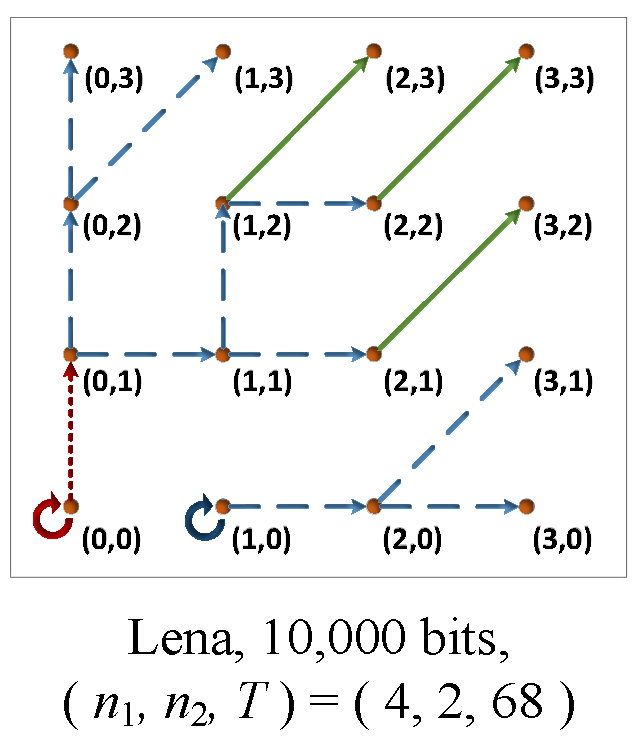
\includegraphics[width=16cm]{1.png}
 \caption{Schematic diagram for detecting frame deletion.}\label{fig:1}
\end{figure*}
It can be seen from figure~\ref{fig:1}. When the 4-EMSSIM algorithm was applied to the forged video, the smooth pattern suffers severe decline which indicates jump-cut caused by frame deletion. After that, we employ a filtering method to extract the abnormal drop of the 4-EMSSIM sequence. Suppose that $b(k)$ represents the result sequence after the calculation of 4-EMSSIM algorithm. $k$ is the index of the corresponding frames. So, $y(k)$ can be get as:
\begin{equation}
y(k)=avg[sum(b(k-N),...,b(k+N))-b(k)]-b(k)
\end{equation}
where $avg[\cdot]$ and $sum(\cdot)$ denote the average and summation of a sequence respectively. $T_1$ is a threshold we set. If $y(k)>T_1$, we consider it a FDP caused by frame deletion.

\subsection{Anti-forensic strategy}
\label{sec:sub22}
As motioned above, the gap between two successive frames at FDP is so large that it can be detected. Accordingly, the principle of anti-forensics maybe to fill the gap. In this way, a simple but reasonable anti-forensic strategy is, frame interpolation at FDP. In the field of video processing, interpolation is widely used to increase the frame rate so as to improve visual quality of video. In figure~\ref{fig:2}, we use $F(x, y, t)$ to represent a video frame sequence, where $x$, $y$ donate spatial coordinates, $t$ is the frame index. The newly interpolated frames are generated in the middle of two adjacent frames by using an algorithm. Let $\alpha$ donates the interpolation times, and $2^{\alpha}-1$ interpolated frames will be added into $F$.

\begin{figure}[!t]
 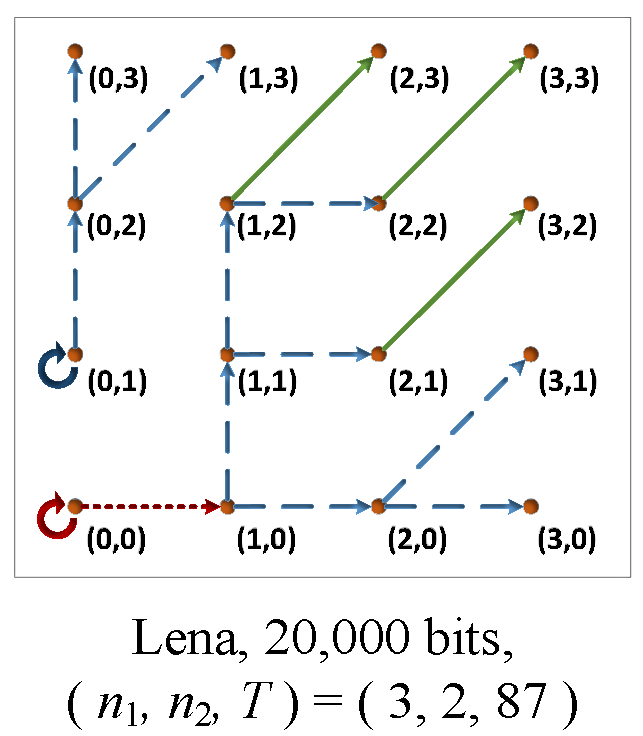
\includegraphics[width=8cm]{2.png}
 \caption{Interpolation diagram in first, second and third time.}\label{fig:2}
\end{figure}

As a specialized video processing technology, many algorithms for video frames interpolation have been proposed before.
Some popular methods like overlapped block motion compensation (OBMC), adaptive OBMC (AOBMC), bidirectional motion estimation (BME), dual weighted based joint OBMC (MCMP) are all motion compensated or motion estimated based. They differ in different motion estimation and compensation strategies. Let us take the AOBMC algorithm as an instance for explanation.
$\hat{F}(x, y, t)$ donates the interpolated frames, $F(x, y, t-1)$ and $F(x, y, t+1)$ are templates for interpolation. The more common circumstance is overlapped block motion compensation.
Suppose that the motion vectors $v_x$ and $v_y$ between two templates are obtained, $l$ blocks overlapped at the interpolation area, then $\hat{F}(x, y, t)$ can be presented as
\begin{multline}
\hat{F}(x, y, t)=\frac{1}{2}\sum_{p=1}^l \omega_p[F(x-v_x, y-v_y, t-1)\\
+F(x+v_x, y+v_y, t+1)]
\end{multline}
Where, $l$ blocks overlapped in the interpolation area,\\ $\sum_{p=1}^l \omega_{p}=1$. For the reason that the videos we concern are with stable background, and there is no moving target between the templates on both sides of the FDP. So, if we ignore the motion vectors in formula (2), it will convert to a simple linear interpolation mode as
\begin{equation}
\hat{F}(x, y, t)=\frac{1}{2}[F(x, y, t-1)+F(x, y, t+1)]
\end{equation}
Because the main difference between these interpolation algorithms is obtaining different motion vectors.
Therefore, all of these interpolation algorithms can be approximated as linear interpolation in the problem we are focus on. We experiment with the AOMBC algorithm in the following.

\section{The detection of anti-forensics}
\label{sec:Thedetection}
%\subsection{Overall description}
%\label{sec:sub31}

In fact, interpolation techniques are main means for videos' frame rate up-conversion which have been discussed in recent years for forensic purpose. Bestagini \emph{et al.} in \cite{A17} provided a feasible method for detecting frame rate up-conversion. The basic idea is that the prediction error of the interpolated frames show periodicity. Furthermore, Ding \emph{et al.} set up an integrated theoretical analysis and method for this problem in \cite{A18}. They employed a spatial and temporal Markov statistics feature to identify different kinds of interpolation algorithms with Error-Correcting Output Code strategy through Ensemble classifier. However, the same opinion of these two schemes is to distinguish interpolated frames and pristine frames with the side-effects caused by motion estimation and compensation. The video frames with stable content will be ignored for the weak residuals. On the contrary, we are focusing on the videos with stable background. Therefore, we did an analysis and proposed a method based on global and local joint feature to detect frame interpolation at FDP.

\subsection{Interpolation analysis}
\label{sec:sub32}

Let us model the interpolation process at FDP. Suppose that $A$ and $B$ are two frames between FDP, and they are the reference frames for interpolation. $A'$ is an original video frame before $A$. Then, $n-1$ interpolated frames $\hat{F}(1),\hat{F}(2),...,\hat{F}(n-1)$ are generated for anti-forensics by using AOBMC algorithm. The interpolation process is shown in figure~\ref{fig:3}. and the video sequences
from $A$ to $B$ can be $$A,\frac{n-1}{n}A+\frac{1}{n}B,...,\frac{1}{2}A+\frac{1}{2}B,...,\frac{1}{n}A+\frac{n-1}{n}B,B$$
if we take a linear model to approximate. So, the gap between two successive interpolated frames $\hat{F}(t)$ and $\hat{F}(t-1)$ is
\begin{equation}
\hat{d}=\hat{F}(t)-\hat{F}(t-1)=\frac{1}{n}(B-A),t\in[1,n-1]
\end{equation}
it can be seen that the gaps of two consecutive frames are related to $A$, $B$ and $n$. As the templets, $A$ and $B$ are consistent. Consequently, if $n$ is large enough, $\hat{d}$ will be rather small. Due to the continuity of video frames as we know, $d$, the gap between $A'$ and $A$ is naturally small. If $\hat{d}$ and $d$ are indistinguishable, the
anti-forensics works.

\begin{figure}[!t]
 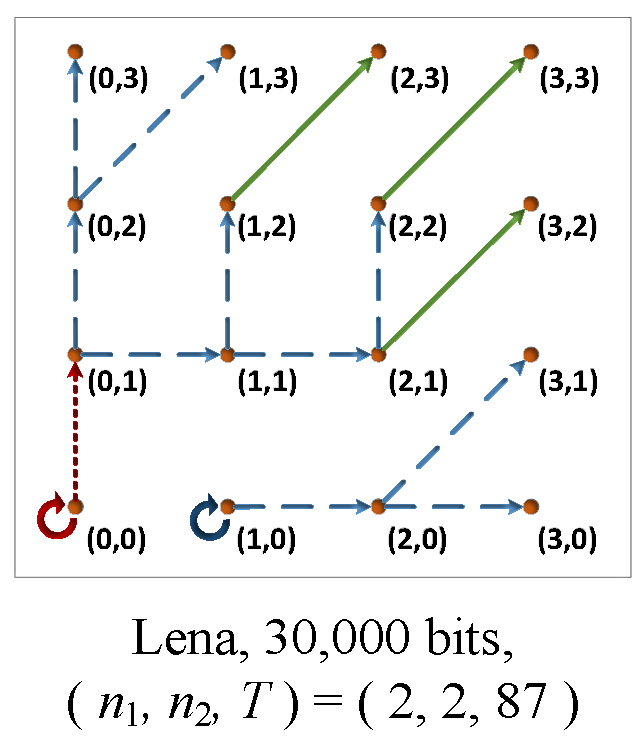
\includegraphics[width=8cm]{3.png}
 \caption{Interpolation diagram at frame deletion point.}\label{fig:3}
\end{figure}
In general, videos are saved in some compressed format. We utilize general video compression framework to make the further analysis. The gap between two frames will directly affect the outcome of motion estimation and compensation in video compression. So, we take the residual of each frame after motion estimation and compensation as the target. Let $\hat{r}$ and $r$ donate interpolated-frame residual and natural-frame residual extracted from the compressed streaming respectively. Combining the forward prediction character of P-frames in videos and the problem we focus, a reasonable suppose we make here is taking $F(t-1)$ (or $\hat{F}(t-1)$) as the motion-estimation reference frame for $F(n)$ (or $\hat{F}(n)$). Thus, $\hat{r}$ and $r$ can be
\begin{equation}
\hat{r}=g(\hat{F}(t),\hat{F}(t-1))=\hat{F}(t)-\hat{F}(t-1)+e(t)\approx\frac{1}{n}(B-A)
\end{equation}
\begin{equation}
r=g(F(t),F(t-1))=F(t)-F(t-1)+e(t)\approx A-A'
\end{equation}
where, $g(\cdot)$ represents the motion compensation, $e(t)$ means the loss of $t-th$ frame caused by quantization.
\begin{figure*}[t!]
\begin{minipage}[t]{0.5\linewidth}
\centering
\subfigure[$r$ in AVC]{\includegraphics[width=7cm]{cover_avc.eps}%
\label{fig:4subfig:a}}
\end{minipage}
\begin{minipage}[t]{0.5\linewidth}
\centering
\subfigure[$\hat{r}$ in AVC]{\includegraphics[width=7.4cm]{stego_avc.eps}%
\label{fig:4subfig:b}}
\end{minipage}
\begin{minipage}[t]{0.5\linewidth}
\centering
\subfigure[$r$ in HEVC]{\includegraphics[width=7cm]{cover_hevc.eps}%
\label{fig:4subfig:c}}
\end{minipage}
\begin{minipage}[t]{0.5\linewidth}
\centering
\subfigure[$\hat{r}$ in HEVC]{\includegraphics[width=7.4cm]{stego_hevc.eps}%
\label{fig:4subfig:d}}
\end{minipage}
\caption{The histograms of $\hat{r}$ and $r$ in H.264/AVC and H.265/HEVC videos}
\label{fig:4}
\end{figure*}

Now, it turns to how to distinguish $\hat{r}$ and $r$. It can be clearly noticed that the interpolated frames are always related to the two templets $A$,$B$ and the interpolated number $n$. The gap between $A$ and $B$ is often very large, while the natural adjacent frames are very similar. We can infer that the distribution of $\hat{r}$ is more complex than $r$.
To confirm our theoretical inferences, we randomly select several pristine frames and interpolated frames to observe the distribution of residuals. The average histograms of $\hat{r}$ and $r$ in H.264/AVC are shown in the figure~\ref{fig:4subfig:a} and figure~\ref{fig:4subfig:b}, one can see that $r$ is concentrated on 0 bin, while $\hat{r}$ is distributed around 0 bin. So, global statistical feature such as SPAM in \cite{A19} can be used to distinguish $\hat{r}$ and $r$ well. However, the situation changes in H.265/HEVC as shown in figure~\ref{fig:4subfig:c} and figure~\ref{fig:4subfig:d}. The difference between $\hat{r}$ and $r$ is not obvious for classification. As the result, the only global statistical feature may not work. In fact, the prediction of coding unit is more accurate in HEVC, so the residuals are more sparse than AVC. In addition, to ensure the real-time performance of the test, the dimensions of feature need to be as low as possible. Therefore, we design a new global and local joint feature to solve this problem.

%There would be detectable difference in the global or local statistics. Combining the some attributes that may be left behind after compression, we proposed a spatial-frequency associated statistical feature.

\subsection{Feature extraction}
\label{sec:sub33}
\subsubsection{global spatial domain statistical feature}
The first feature is derived from the following assumption that the residual $\hat{r}$ and $r$ follow the different distributions. As the result, it is possible to capture their statistical descriptions by using probability mass function. The prior knowledge and lots of observations tell us that the value of residual is generally small, and cluster around zero. In our work, we set a threshold $T_2$ and calculate the probability for $r(x, y)$ belongs to $[-T_2...T_2]$. if $r(x, y)$ is larger than $T_2$ or smaller than $-T_2$, $r(x, y)$ will be set to $T_2$ or $-T_2$. So,
\begin{equation}
H(i)=\frac{1}{N_x N_y}\sum_{x=1}^{N_x} \sum_{y=1}^{N_y} \delta[i-r(x,y)]
\end{equation}
$N_x$,$N_y$ are residual's size which is the same as the video. $\delta$ is the Kronecker delta. $i\in[-T_2...T_2]$, and in
this paper we set $T_2=5$. Therefore, $H(i)$ is a 11-D feature vector.

\subsubsection{global frequency domain statistical feature}
Because the global distribution of the spatial domain is not powerful enough to capture all the information, we carry on extracting global feature in frequency domain. In the most popular and most advanced video compression standards, the smallest coding units are all 4x4 blocks. As a consequence, we divide the residual matrix into non-overlapped 4x4 blocks.
Thus, useful feature is generated after employing DCT transform on the 4x4 blocks. For a fixed DCT mode $(m, n)$, let $h_{m,n}(i)$ donates the feature vector
\begin{equation}
h_{m,n}(i)=\frac{1}{N_B}\sum_{p=1}^{N_B} \delta\{i-dct[r(m,n,p)]\}
\end{equation}
where $N_B$ is the number of blocks in per frame, $p\in[1...N_B]$ represents $p-th$ block in per frame. we set $m,n\in[1,2,3]$
, and $3\leq m+n \leq5$. For the integrity of DCT coefficient, we set $i\in[-3,-2.5...2.5,3]$ in formula(8).

\begin{figure*}[tb]
\subfigure[Scene 1]{\includegraphics[width=4cm]{scene1.png}%
\label{fig:subfig:a}}
\hfil
\subfigure[Scene 2]{\includegraphics[width=4cm]{scene2.png}%
\label{fig:subfig:b}}
\hfil
\subfigure[Scene 3]{\includegraphics[width=4cm]{scene3.png}%
\label{fig:subfig:c}}
\hfil
\subfigure[Scene 4]{\includegraphics[width=4cm]{scene4.png}%
\label{fig:subfig:d}}
\hfil
\caption{indoor and outdoor scenes in the video database}
\label{fig:5}
\end{figure*}

\subsubsection{Local inter-block difference feature}
The next feature is based on the fact that artificial interpolation add entropy to the quantized DCT coefficients of
residuals. The confusion of residuals results that the encoder chooses smaller blocks in the coding process to achieve
accurate prediction. The dependences between two adjacent 4x4 blocks are calculated using a variation indicator as
\begin{multline}
V=\frac{\sum_{x=1}^{4\lceil \frac{N_x}{4} \rceil-4} \sum_{y=1}^{4\lceil\frac{N_y}{4}\rceil}|d(x,y)-d(x+4,y)|}{16(\lceil \frac{N_x}{4} \rceil-1)\lceil \frac{N_y}{4} \rceil} \\
+\frac{\sum_{x=1}^{4\lceil \frac{N_x}{4} \rceil} \sum_{y=1}^{4\lceil\frac{N_y}{4}\rceil-4}|d(x,y)-d(x,y+4)|}{16\lceil \frac{N_x}{4} \rceil(\lceil \frac{N_y}{4} \rceil-1)}
\end{multline}
where $d$ is the coefficient matrix after 4x4 DCT transform, $N_x$ and $N_y$ are the height and width of residual.

\subsubsection{Local block boundary difference feature}
Another metric to describe the dependency of inter-block is discontinuity which is defined as the sum of the blocks' boundary in the spatial domain. We expect that the interpolation would increase the discontinuity rather than reduction. There are two measures for $\gamma=1$ and $\gamma=2$
\begin{multline}
B_{\gamma}=\frac{\sum_{x=1}^{\lfloor \frac{N_x-1}{4} \rfloor} \sum_{y=1}^{ N_y }|r(4x,y)-r(4x+1,y)|^{\gamma}}{N_y \lfloor \frac{N_x-1}{4} \rfloor + N_x \lfloor \frac{N_y-1}{4} \rceil} \\
+\frac{\sum_{x=1}^{N_x} \sum_{y=1}^{\lfloor \frac{ N_y -1}{4} \rfloor}|r(x,4y)-r(x,4y+1)|^{\gamma}}{N_y \lfloor \frac{N_x-1}{4} \rfloor + N_x \lfloor \frac{N_y-1}{4} \rceil}
\end{multline}
where $N_x$ and $N_y$ are the height and width of residual. The features extracted from four aspects above are summarized in Table~\ref{table:1}.

\begin{table}[t]
% increase table row spacing, adjust to taste
\renewcommand{\arraystretch}{1.3}
% if using array.sty, it might be a good idea to tweak the value of
% \extrarowheight as needed to properly center the text within the cells
\caption{79-D global and local associated feature}
\label{table:1}
\begin{tabular}{cccc}
\hline
Feature name & Notation & Range & Dimensions\\
\noalign{\smallskip}\hline\noalign{\smallskip}
Spatial & $H(i)$ & $-5\leq i \leq5$ & 11\\
Frequency & $h_{m,n}(i)$ & $3\leq m+n \leq5$, $\left| i \right| \leq3$ & $13\times5$\\
Variation & $V$ & * & 1\\
Blockiness & $B_{\gamma}$ & * & 2\\
\hline
\end{tabular}
\end{table}

\section{Experiments and results}
\label{sec:experiments}
\subsection{database setup}

\label{sec:10}
To verify the anti-forensic methods and the feature we proposed for detecting anti-forensics, we established two new video datasets in this paper. There are a total of 100 original surveillance videos recoded from four different scenes as shown in figure~\ref{fig:5}. The resolution of each video is CIF (352x288). The selection of the scenes contains different factors such as indoor or outdoor, complexity of the background, the intensity of light. And we removed some key frames which contain the appearance of targets, so each video contains one FDP. These 100 tampered videos will be employed as the basic data to conduct all the experiments in this paper.

\subsection{frames deletion anti-forensics}
\label{sec:11}
Since we think that the inter-frame continuity based frames deletion forensic methods could be easily attacked by frames interpolation at FDP, we will evaluate this anti-forensic idea in this part. To start with the parameter $\alpha$ of interpolation. In general, the number of interpolated frames $n$ for anti-forensics can be 0,1,3,7,15,31,63,... ($n=2^\alpha-1$, where $\alpha=0,1,2,3,4,5,6,...$) in terms of the interpolation algorithm reported in figure~\ref{fig:2}. The interpolation needs to be conducted in pixel domain, the anti-forensic videos are then re-coded with high-quality compressed format. Unlike the common indicators in classification problem, we define the detection accuracy (DA) ratio and FDP location false alarm (LFA) ratio in these anti-forensics experiments as the indicators. Due to the inter-frame continuity based methods are capable to precisely locate PDF, indicators should also involve the location performance. Two indicators are defined as :
\begin{equation}
DA\ ratio=\frac{N_a}{N}
\end{equation}
\begin{equation}
LFA\ ratio=\frac{N_l}{N}
\end{equation}

where $N$ is the total number of after-anti-forensics videos ($N=100$ in our test), $N_a$ is the number of videos which have been correctly exposed to be frames-deleted by the inter-frame continuity based methods and $N_l$ is the number of videos which are misdiagnosed with the position of FDP. One situation is if the test certainly pick out the real FDP as well as some false FDPs, we think it a valid frame deletion detection, but also a contribution to location false alarm as well. Two inter-frame continuity based methods optical flow in \cite{A10} and 4-EMSSIM in \cite{A12} are employed to run the tests. As mentioned before, such frames deletion test algorithm needs a threshold to judge FDP or not. We use three thresholds {0.005 0.007 0.01} in optical flow method and two thresholds {0.0085 0.005} in 4-EMSSIM to do the tests. The results of these two forensic methods under different $\alpha$ (the max $\alpha$ we set in this paper is 6, so the max interpolation number is 63) can be seen in figure~\ref{fig:6} and figure~\ref{fig:7}.

We notice that when the number of interpolated frames is 0 (no anti-forensics), two forensic methods can achieve a very high detection accuracy with a relatively low location false alarm. However, serious drop of detection accuracy appear when the number of interpolated frames is larger than 3. Meanwhile, the location false alarm gets worse as well. In light of this, three or more interpolated frames at FDP can make the inter-frame continuity based methods almost ineffective to detect frame deletion which shows the validity of the anti-forensic strategy we proposed. Consider that the frame rate in videos is usually 25 or 30 frames per second, even 63 frames' interpolation at FDP will only increase the duration of the video by 2 seconds. In a word, the experiments prove the threat of anti-forensics we proposed needs attention.

\subsection{the detection of anti-forensics}
\label{sec:sub41}
In this part, the performance of our proposed detector towards anti-forensics will be shown. As a matter of fact, compression is always necessary for videos' storage. For the sake of exploring the influence of diverse codec parameters to the detector, we use the two most popular video compression standards H.264/AVC and H.265/HEVC to provide video compression for the experiments. We utilize three constant bitrates (400,700,1000 kb/s) as low, medium and high quality of compression for CIF videos, which are the general settings in daily life. From the result of~\ref{sec:11}, we can see that when the number of interpolated frames exceeds 7, the forensic method for frame deletion is invalid. So we first picked out the four cases $n=7,15,31,63$ of the interpolated number to verify the proposed feature.

\begin{figure}[!t]
 \includegraphics[width=8.5cm]{figure5.eps}
 \caption{Detection accuracy ratio under different interpolation parameters.}\label{fig:6}
\end{figure}

\begin{figure}[!t]
 \includegraphics[width=8.5cm]{figure6.eps}
 \caption{FDP location false alarm ratio under different interpolation parameters.}\label{fig:7}
\end{figure}

As analyzed in Section~\ref{sec:Thedetection}, our detector employs the features extracted from the residual in P frames. To increase the number of available P frames in a single video, we encode all the AVC and HEVC videos in baseline profile with only I frames and P frames in the videos. Combined with the parameters mentioned above and 100 original videos, a total of 2400 videos were built as dataset1. The parameter setting of dataset1 is summarized in Table~\ref{table:2}.
\begin{table}[t]
\renewcommand\arraystretch{1.5}
    \caption{The parameter setting of dataset1}\label{table:2}
    \begin{center}
        \begin{tabular*}{7cm}{cc}
            \hline
            \ & Parameter setting\\
            \noalign{\smallskip}\hline\noalign{\smallskip}
            Codec & H.264/AVC,H.265/HEVC  \\
            Bitrate(kb/s) & 400,700,1000  \\
            inserted algorithm & AOMBC  \\
            inserted number & 7,15,31,63 frames\\
            GOP size & 250 (codec default)
            \\ \hline
        \end{tabular*}
    \end{center}
\end{table}
After an exhaustive investigation, we don't find any exact work for the same purpose with our paper. As a result, we utilize a 98 dimensional SPAM feature \cite{A19} as the comparison which is similar with the Markov feature used in \cite{A18}. Table~\ref{table:3} and Table~\ref{table:4} show the experimental results of videos coded with AVC and HEVC respectively. As mentioned before, the detection of anti-forensics is to distinguish pristine frames and interpolated frames. Each accuracy rate under the corresponding parameter is obtained by training and test. Pristine frames and interpolated frames are used as negative and positive samples. Half of all samples are employed to train the parameters of the classifier. Another half of the samples are utilized for test. The final test accuracy rate is the average result of ten random selections of training and test sets by the Ensemble Classifier.
\begin{table*}[b]
\renewcommand\arraystretch{1.5}
    \caption{Performance in H.264/AVC videos(\%)}\label{table:3}
    \begin{center}
        \begin{tabular*}{14.5cm}{ccccccccccccc}
            \hline
            \ & \multicolumn{3}{c}{scene1} & \multicolumn{3}{c}{scene2} & \multicolumn{3}{c}{scene3} &\multicolumn{3}{c}{scene4} \\ \cline{2-4}\cline{5-7}\cline{8-10}\cline{11-13}
            bitrate & 400 & 700 & 1000 & 400 & 700 & 1000 & 400 & 700 & 1000 & 400 & 700 & 1000 \\ \hline
            7-Ours & 99.66 & 100.0 & 99.48 & 100.00 & 100.0 & 100.0 & 100.0 & 100.0 & 100.0 & 100.0 & 100.0 & 100.0 \\
            7-Spam & 99.60 & 100.0 & 100.0 & 100.00 & 100.0 & 100.0 & 100.0 & 100.0 & 100.0 & 100.0 & 100.0 & 100.0 \\ \hline
            15-Ours & 98.93 & 99.36 & 99.84 & 100.00 & 99.87 & 99.63 & 98.53 & 99.73 & 99.60 & 100.0 & 100.0 & 100.0 \\
            15-Spam & 99.30 & 99.73 & 100.0 & 100.00 & 99.97 & 100.0 & 98.74 & 99.87 & 99.73 & 100.0 & 100.0 & 100.0 \\ \hline
            31-Ours & 99.57 & 99.96 & 99.77 & 98.02 & 97.89 & 97.78 & 92.51 & 95.10 & 96.64 & 96.63 & 98.42 & 98.20 \\
            31-Spam & 99.61 & 99.77 & 99.87 & 97.14 & 97.74 & 98.41 & 93.04 & 95.16 & 96.81 & 96.50 & 97.52 & 98.07 \\ \hline
            63-Ours & 99.36 & 99.74 & 99.65 & 98.02 & 97.55 & 98.63 & 91.97 & 90.72 & 93.51 & 94.75 & \textbf{96.09} & 94.61 \\
            63-Spam & 99.68 & 99.76 & 99.56 & 98.08 & \textbf{98.65} & 99.47 & 95.55 & \textbf{92.85} & 93.64 & 93.53 & 93.57 & 94.88
            \\ \hline
        \end{tabular*}
    \end{center}
\end{table*}

\begin{table*}[b]
\renewcommand\arraystretch{1.5}
    \caption{Performance in H.265/HEVC videos(\%)}\label{table:4}
    \begin{center}
        \begin{tabular*}{14.5cm}{ccccccccccccc}
            \hline
            \ & \multicolumn{3}{c}{scene1} & \multicolumn{3}{c}{scene2} & \multicolumn{3}{c}{scene3} &\multicolumn{3}{c}{scene4} \\ \cline{2-4}\cline{5-7}\cline{8-10}\cline{11-13}
            bitrate & 400 & 700 & 1000 & 400 & 700 & 1000 & 400 & 700 & 1000 & 400 & 700 & 1000 \\ \hline
            7-Ours & 98.91 & 98.39 & 98.74 & \textbf{97.70} & \textbf{97.70} & 95.40 & 100.0 & 99.02 & 99.02 & 99.37 & 97.36 & 97.70 \\
            7-Spam & 99.07 & \textbf{99.77} & 98.28 & 96.44 & 95.40 & 94.89 & 100.0 & 99.37 & 99.37 & 98.85 & 97.64 & 97.70 \\ \hline
            15-Ours & 98.53 & 94.57 & 96.66 & \textbf{93.24} & 93.34 & \textbf{93.37} & 98.96 & 98.10 & 97.64 & \textbf{95.91} & 99.65 & 99.09 \\
            15-Spam & 98.96 & 94.87 & 96.52 & 90.13 & 93.34 & 92.11 & 98.68 & 99.04 & \textbf{99.73} & 94.49 & 99.28 & 99.07 \\ \hline
            31-Ours & \textbf{98.29} & 96.16 & 95.67 & 90.36 & \textbf{90.32} & 90.16 & 90.05 & \textbf{92.34} & \textbf{92.74} & 93.06 & \textbf{93.79} & \textbf{95.47} \\
            31-Spam & 96.89 & 95.50 & 95.04 & 89.74 & 87.93 & 89.78 & \textbf{92.84} & 90.61 & 91.59 & 93.02 & 92.53 & 94.26 \\ \hline
            63-Ours & 97.02 & 94.82 & 94.38 & 84.64 & \textbf{85.65} & \textbf{84.53} & 81.13 & 83.84 & 82.81 & \textbf{87.54} & 78.44 & \textbf{82.23} \\
            63-Spam & 97.55 & 94.11 & 94.15 & 85.06 & 83.16 & 81.89 & 82.59 & 83.97 & 82.95 & 86.52 & 78.75 & 80.07
            \\ \hline
        \end{tabular*}
    \end{center}
\end{table*}
The experimental results will be analyzed from the following different perspectives. As one can see, the performance of our proposed feature is approximately the same with the SPAM in AVC videos. Note that our proposed feature's dimension is 1/4 less than SPAM. As to the HEVC videos, the proposed feature performs better than SPAM as shown in Table~\ref{table:4}. The results also verify our previous analysis in~\ref{sec:sub32}. The residuals in HEVC are more sparse than AVC. As a result, the global feature such as SPAM can not work well. Therefore, the proposed local inter-block and block boundary difference feature can capture the anomalies between the pristine frame and the interpolated frame more effectively. On the contrary, SPAM with the help of histograms of Markov transition probability matrix are blindfold to a certain extent.

When the interpolated number of frames is added at FDP, the accuracy of detection drops slightly. It is reasonable for the artifacts left by interpolation are getting weaker after being averaged
to more frames. Obviously, the detection results of AVC videos are generally higher than HEVC videos in the same parameter if Table~\ref{table:3} and Table~\ref{table:4} are compared. The main reason is that HEVC does well in motion estimation and compensation, the features based on
the residual gets weaker in both indoor and outdoor videos. As for the influence of different bitrates,
high bitrate videos perform better in AVC videos, but not obvious in HEVC videos. In a word, the experimental results show that the proposed feature is effective for distinguishing the pristine frames and interpolated frames.

\subsection{mixed training and test}
Although the content and bitrate can be obtained from the investigated video, we do not know whether the video is interpolated at a certain location or how many frames are interpolated. Note that any number of frames can be inserted at FDP as long as anti-forensics is valid, the detector needs to deal with a variety of situations. We use all the frames in dataset1 under certain bitrate and scene as the samples for mixed training. In order to verify the effectiveness of our feature in other interpolated cases. We create dataset2 for test in which the interpolated frames are generated by AOBMC algorithm with $n = 10,23,45$. These three numbers are randomly selected for interpolation. Details of dataset2 are shown in Table~\ref{table:5}.

\begin{table}[h]
\renewcommand\arraystretch{1.5}
    \caption{The parameter setting of dataset2}\label{table:5}
    \begin{center}
        \begin{tabular*}{7cm}{cc}
            \hline
            \ & Parameter setting\\
            \noalign{\smallskip}\hline\noalign{\smallskip}
            Codec & H.264/AVC,H.265/HEVC  \\
            Bitrate(kb/s) & 400,700,1000  \\
            inserted algorithm & AOMBC  \\
            inserted number & 10,23,45 frames\\
            GOP size & 250 (codec default)
            \\ \hline
        \end{tabular*}
    \end{center}
\end{table}

The result of mixed training and test is shown in Table~\ref{table:6} for AVC and Table~\ref{table:7} for HEVC. Although the performance of proposed cannot do better than the SPAM feature in AVC videos, the proposed performs better than SPAM in HEVC videos as shown in Table~\ref{table:7}. The reason is the same as mentioned in ~\ref{sec:sub41}. Despite the comparison, our proposed method are capable to distinguish interpolated and pristine frames effectively with a mixed trained detector.

\begin{table*}[b]
\renewcommand\arraystretch{1.5}
    \caption{Mixed training and test in H.264/AVC videos(\%).}\label{table:6}
    \begin{center}
        \begin{tabular*}{14.5cm}{ccccccccccccc}
            \hline
            \ & \multicolumn{3}{c}{scene1} & \multicolumn{3}{c}{scene2} & \multicolumn{3}{c}{scene3} &\multicolumn{3}{c}{scene4} \\ \cline{2-4}\cline{5-7}\cline{8-10}\cline{11-13}
            bitrate & 400 & 700 & 1000 & 400 & 700 & 1000 & 400 & 700 & 1000 & 400 & 700 & 1000 \\ \hline
            10-Ours & 98.00 & 99.00 & 99.00 & 95.00 & 96.00 & 100.0 & 88.00 & 95.00 & 98.00 & 90.00 & 98.00 & 97.00 \\
            10-Spam & 100.0 & 100.0 & 100.0 & 99.00 & 100.0 & 100.0 & 95.00 & 97.00 & 97.00 & 88.00 & 99.00 & 95.00 \\ \hline
            23-Ours & 99.13 & 98.70 & 99.13 & 98.26 & 97.87 & 98.70 & 91.30 & 91.74 & 97.39 & 95.22 & 97.39 & 96.96 \\
            23-Spam & 99.57 & 100.0 & 100.0 & 99.13 & 100.0 & 100.0 & 90.87 & 96.52 & 97.39 & 95.06 & 97.39 & 98.22 \\ \hline
            45-Ours & 98.89 & 98.89 & 98.70 & 96.89 & 97.56 & 98.67 & 89.56 & 91.56 & 93.78 & 92.44 & 96.89 & 94.89\\
            45-Spam & 99.33 & 99.78 & 99.56 & 96.44 & 99.11 & 100.0 & 90.22 & 92.00 & 94.67 & 89.11 & 93.56 & 94.89
            \\ \hline
        \end{tabular*}
    \end{center}
\end{table*}

\begin{table*}[b]
\renewcommand\arraystretch{1.5}
    \caption{Mixed training and test in H.265/HEVC videos(\%).}\label{table:7}
    \begin{center}
        \begin{tabular*}{14.5cm}{ccccccccccccc}
            \hline
            \ & \multicolumn{3}{c}{scene1} & \multicolumn{3}{c}{scene2} & \multicolumn{3}{c}{scene3} &\multicolumn{3}{c}{scene4} \\ \cline{2-4}\cline{5-7}\cline{8-10}\cline{11-13}
            bitrate & 400 & 700 & 1000 & 400 & 700 & 1000 & 400 & 700 & 1000 & 400 & 700 & 1000 \\ \hline
            10-Ours & 99.00 & 95.00 & 96.00 & 85.00 & 92.00 & 89.00 & 97.00 & 95.00 & 88.00 & 92.00 & 92.00 & 96.00 \\
            10-Spam & 94.00 & 91.00 & 93.00 & 92.00 & 91.00 & 87.00 & 95.00 & 92.00 & 90.00 & 93.00 & 92.00 & 95.00 \\ \hline
            23-Ours & 97.83 & 93.04 & 95.22 & 89.57 & 90.87 & 90.87 & 94.35 & 93.91 & 94.35 & 94.35 & 92.61 & 94.35 \\
            23-Spam & 97.39 & 94.78 & 95.65 & 92.17 & 87.83 & 93.04 & 94.35 & 92.17 & 90.87 & 93.91 & 93.04 & 91.30 \\ \hline
            45-Ours & 97.33 & 97.56 & 95.56 & 81.33 & 81.11 & 80.00 & 89.56 & 93.33 & 91.11 & 87.56 & 84.22 & 87.11\\
            45-Spam & 96.44 & 93.56 & 95.33 & 78.22 & 78.00 & 78.44 & 89.11 & 91.56 & 91.33 & 86.89 & 84.22 & 86.22
            \\ \hline
        \end{tabular*}
    \end{center}
\end{table*}

\subsection{blind test for video}
\begin{figure}[!t]
 \includegraphics[width=8.5cm]{fig10.eps}
 \caption{The votes of each frame judged as interpolated, the horizontal axis represents the index of frame in a video, and the vertical axis is the votes.}\label{fig:10}
\end{figure}

\begin{figure}[!t]
 \includegraphics[width=8.5cm]{fig12.eps}
 \caption{The blind test result after filtering-like two-step operation. The figure indicates there are interpolation from 78-th to 122-th frame, and the individual spikes are more likely false alarm, and have been removed}\label{fig:11}
\end{figure}

\begin{figure*}[tp]
\begin{minipage}[t]{0.5\linewidth}
\centering
\subfigure[overlap=0.9393]{\includegraphics[width=6.1cm]{avc09393.png}%
\label{fig:subfig:a}}
\end{minipage}
\begin{minipage}[t]{0.5\linewidth}
\centering
\subfigure[overlap=0.8665]{\includegraphics[width=6.1cm]{avc08665.png}%
\label{fig:subfig:b}}
\end{minipage}
\begin{minipage}[t]{0.5\linewidth}
\centering
\subfigure[overlap=0.7046]{\includegraphics[width=6.1cm]{avc07046.png}%
\label{fig:subfig:c}}
\end{minipage}
\begin{minipage}[t]{0.5\linewidth}
\centering
\subfigure[overlap=0.6522]{\includegraphics[width=6.1cm]{avc06522.png}%
\label{fig:subfig:d}}
\end{minipage}
\caption{The blind test results of H.264/AVC videos.}
\label{fig:8}
\end{figure*}

\begin{figure*}[tp]
\begin{minipage}[t]{0.5\linewidth}
\centering
\subfigure[overlap=0.9667]{\includegraphics[width=6.1cm]{hevc09667.png}%
\label{fig:subfig:a}}
\end{minipage}
\begin{minipage}[t]{0.5\linewidth}
\centering
\subfigure[overlap=0.8674]{\includegraphics[width=6.1cm]{hevc08674.png}%
\label{fig:subfig:b}}
\end{minipage}
\begin{minipage}[t]{0.5\linewidth}
\centering
\subfigure[overlap=0.7110]{\includegraphics[width=6.1cm]{hevc07110.png}%
\label{fig:subfig:c}}
\end{minipage}
\begin{minipage}[t]{0.5\linewidth}
\centering
\subfigure[overlap=0.6272]{\includegraphics[width=6.1cm]{hevc06272.png}%
\label{fig:subfig:d}}
\end{minipage}
\caption{The blind test results of H.265/HEVC videos.}
\label{fig:9}
\end{figure*}

The detection of anti-forensics is to diagnose videos for integrity. We utilize the mixed trained detector, and randomly select videos in dataset2 as the research objects to do blind test in this part. The classifier we use in this paper is the Ensemble Classifiers which consists of many base learners independently trained on a set of positive and negative samples. So, the classification result of each test sample is determined by the votes of all base learners. As shown in figure~\ref{fig:10}, the horizontal axis represents the index of frame in a video, and the vertical axis is the votes. The votes are obtained by adding +1 or -1 by each base learner. Consider that the judgement with less votes nearby 0 vote is not reliable. And from prior knowledge, the interpolated frames are always appear continuously, isolated spikes can be identified as misjudgement. Assume $v_i$ indicates the votes of i-th frame and $N_c$ represents the number of base learners, we utilize a filtering-like two-step operation
\begin{equation}
v_i=\left\{
\begin{array}{lc}
0,\  if\  v_i<0.6\cdot N_c\\
v_i,\  otherwise\\
\end{array}
\right.
\end{equation}
\begin{equation}
v_i=\left\{
\begin{array}{lc}
0,\  if\  v_i-(v_{i-1}+v_{i+1})/2>0.9\cdot v_i\\
v_i,\  otherwise\\
\end{array}
\right.
\end{equation}
then the figure~\ref{fig:11} is the blind test result for a video. Therefore, we exhibit some detection result of AVC and HEVC videos in figure~\ref{fig:8} and figure~\ref{fig:9}. As one can see, the frames between the two red dotted lines in the figure is the ground truth of interpolation. Although some frames with fewer votes are misjudged as pristine frames, it will not impact the overall judgment. From these figures, the interpolated parts can be clearly seen and located.

In order to measure the performance of blind test, we use the overlap between detection result and ground truth which is defined as follows:
\begin{equation}
overlap=\frac{N_{in}}{G}-\frac{N_{out}}{N_t-G}
\label{formula:14}
\end{equation}
where $G$ represents the number of frames in the interpolation ground truth sequence, $N_t$ is the total number of frames for a single video. $N_{in}$ indicates the number of frames that are correctly judged to be interpolated. And $N_{out}$ is the number of frames wrongly judged to be interpolated. Large overlap value means the detection result is accurate. And then, we use the overlap to verify the performance of our proposed method in blind test from different aspects. In Table~\ref{table:8}, as one can see, the overlap decreases in outdoor scenes especially in HEVC videos. The average overlap of HEVC videos dropped to 0.6883, but according to figure~\ref{fig:8} and figure~\ref{fig:9}, the existence of interpolated frames can be visually detected even the overlap dropped to 0.6.

In Table~\ref{table:9}, the blind test were done in three different bitrates. The experimental result shows that our proposed method does not depend on a fixed bitrate. The performances are similar at low, medium and high bitrates. Table~\ref{table:10} shows that the result of 10 frames interpolation is the worst in three cases. The reason is that the misjudgement over 10 frames will have a great impact on overlap from the formula~\ref{formula:14}. Furthermore, the result of 45 frames interpolation is slightly worse than the result of 23 frames. It's reasonable because the more frames are inserted, the weaker the traces left. The result of AVC videos are better than HEVC. As the most advanced video coding scheme, HEVC's block strategy is more refined and motion estimation is more accurate, which results in more sparse residuals. Then the feature based on residual of frames we proposed will be affected. To sum up, the proposed method can detect the frame-interpolation parts in a video effectively, which indicates the video may experienced frame deletion at a certain point.
\begin{table}[h]
\renewcommand\arraystretch{1.5}
    \caption{The average results of overlap in different scenes.}\label{table:8}
        \begin{tabular*}{7cm}{ccccc}
            \hline
            \ & scene1 &scene2 & scene3 &scene4 \\
            \noalign{\smallskip}\hline\noalign{\smallskip}
            AVC & 0.9667 & 0.9035 & 0.8291 & 0.8996  \\
            HEVC & 0.9116 & 0.7086 & 0.7964 & 0.6883
            \\ \hline
        \end{tabular*}
\end{table}
\begin{table}[h]
\renewcommand\arraystretch{1.5}
    \caption{The average results of overlap in different bitrates.}\label{table:9}
        \begin{tabular*}{6cm}{cccc}
            \hline
            \ & 400 kb/s & 700 kb/s & 1000 kb/s \\
            \noalign{\smallskip}\hline\noalign{\smallskip}
            AVC & 0.8753 & 0.8982 & 0.9256 \\
            HEVC & 0.8044 & 0.7789 & 0.7425
            \\ \hline
        \end{tabular*}
\end{table}
\begin{table}[h]
\renewcommand\arraystretch{1.5}
    \caption{The average results of overlap in different interpolations.}\label{table:10}
        \begin{tabular*}{6cm}{cccc}
            \hline
            \ & insert10 & insert23 & insert45 \\
            \noalign{\smallskip}\hline\noalign{\smallskip}
            AVC & 0.8673 & 0.9339 & 0.8979 \\
            HEVC & 0.8016 & 0.8153 & 0.7089
            \\ \hline
        \end{tabular*}
\end{table}
%\begin{acknowledgements}
%If you'd like to thank anyone, place your comments here
%and remove the percent signs.
%\end{acknowledgements}

% BibTeX users please use one of
%\bibliographystyle{spbasic}      % basic style, author-year citations
%\bibliographystyle{spmpsci}      % mathematics and physical sciences
%\bibliographystyle{spphys}       % APS-like style for physics
%\bibliography{}   % name your BibTeX data base
\section{Conclusion}
\label{sec:Conclusion}
In the forensics of video frame deletion, even the inter-frame continuity based methods such as optical flow, speed field and human visual-inspired measure are effective to detect and locate frame deletion, they can also be easily attacked by anti-forensic technique. In this paper, we first proposed an anti-forensic scheme with high probability to appear. That is, conducting the inter-frame interpolation at the frame deletion point (FDP). By using the two frames on both sides of FDP as templates, the frames generated by interpolation can repair the inter-frame continuity with no visual artifact. The experimental results show that all the three forensic methods fail once the anti-forensic technique is applied.

In order to deal with this potential anti-forensic technique, we then put forward a global and local joint feature to distinguish the interpolated frame from the pristine frame in a video. The feature makes full use of some local artifacts and overcomes the problem of weak residual in HEVC videos. Complete experiments show that the detectors trained with different kinds of interpolated frames can correctly detect the presence of interpolated frames in the test video. Therefore, the method we proposed is effective to detect and locate the frame deletion under anti-forensics.

\begin{thebibliography}{}
%
% and use \bibitem to create references. Consult the Instructions
% for authors for reference list style.
%
\bibitem{A1}
% Format for Journal Reference
A. Piva, An Overview on Image Forensics, ISRN Signal Processing (2013)
\bibitem{A2}
% Format for Journal Reference
P. Bestagini, M. Fontani, S. Milani, M. Barni, A. Piva, M. Tagliasacchi and S. Tubaro, An Overview On Video Forensics, in the 20th European Signal Processing Conference (2012)
\bibitem{A3}
% Format for Journal Reference
R.D. Singh and N. Aggarwal, Video content authentication techniques: acomprehensive survey, Multimedia Systems, pp. 1-30 (2017)
\bibitem{A4}
% Format for Journal Reference
W. Wang and H. Farid, Exposing digital forgeries in video by detecting double MPEG compression, in 8th ACM workshop on Multimedia and security, pp. 37-47 (2006)
\bibitem{A5}
% Format for Journal Reference
W. Luo, M. Wu, and J. Huang, Mpeg recompression detection based on block artifacts, in SPIE 6819, Security, Forensics, Steganography, and Watermarking of Multimedia Contents X. SPIE, pp. 68190X-68190X-12 (2008)
\bibitem{A6}
% Format for Journal Reference
T. Shanableh, Detection of frame deletion for digital video forensics, Digital Investigation, vol. 10, no. 4, pp. 350-360 (2013)
\bibitem{A7}
% Format for Journal Reference
D. V{\'a}zquez-Pad{\'i}n, M. Fontani, T. Bianchi, P. Comesana, A. Piva, and M. Barni, Detection of video double encoding with gop size estimation, in IEEE International Workshop on Information Forensics and Security, pp. 151-156 (2012)
\bibitem{A8}
% Format for Journal Reference
A Gironi, M Fontani, T Bianchi, A Piva, M Barni, A video forensic technique for detecting frame deletion and insertion, in IEEE International Conference on Acoustics, Speech and Signal Processing, pp. 6226-6230 (2014)
\bibitem{A9}
% Format for Journal Referenc
C. Feng, Z. Xu, S. Jia, W. Zhang, and Y. Xu, Motion adaptive frame deletion detection for digital video forensics, IEEE Transactions on Circuits and Systems for Video Technology, vol. 27, no. 12, pp. 2543-2554 (2017)
\bibitem{A10}
% Format for Journal Reference
J. Chao, X. Jiang, and T. Sun, A novel video inter-frame forgery model detection scheme based on optical flow consistency, in International Workshop on Digital Forensics and Watermarking, pp. 267-281 (2013)
\bibitem{A11}
% Format for Journal Reference
Y. Wu, X. Jiang, T. Sun, and W. Wang, Exposing video inter-frame forgery based on velocity field consistency, in IEEE International Conference on Acoustics, Speech and Signal Processing, pp. 2674-2678 (2014)
\bibitem{A12}
% Format for Journal Reference
Q. Wan, K. Panetta, S. Agaian, A video forensic technique for detecting frame integrity using human visual system-inspired measure, in IEEE International Symposium on Technologies for Homeland Security, pp. 1-6 (2017)
\bibitem{A13}
% Format for Journal Reference
 M. Kirchner and R. Bohme, Hiding traces of resampling in digital images, IEEE Transactions on Information Forensics and Security, vol 3, no 4, pp. 582-592 (2008)
 \bibitem{A14}
% Format for Journal Reference
G. Cao, Y. Zhao, R. Ni and H. Tian, Anti-forensics of contrast enhancement in digital images, in Proceedings of 12th ACM Workshop on Multimedia and Security, pp. 25-34 (2010)
 \bibitem{A15}
% Format for Journal Reference
M.C. Stamm, W.S. Lin and K.J.R. Liu, Temporal forensics and anti-forensics for motion compensated video. IEEE Transactions on Information Forensics and Security, vol 7, no 4, pp. 1315-1329 (2012)
\bibitem{A16}
% Format for Journal Reference
X. Kang, J. Liu, H. Liu and Z. Wang, Forensics and counter anti-forensics of video inter-frame forgery, Multimedia Tools and Applications, vol 75, no 21, pp. 13833-13853 (2016)
\bibitem{A17}
% Format for Journal Reference
P. Bestagini, S. Battaglia, S. Milani, M. Tagliasacchi, and S. Tubaro, Detection of temporal interpolation in video sequences, in IEEE International Conference on Acoustics, Speech and Signal Processing, pp. 3033-3037 (2013)
\bibitem{A18}
% Format for Journal Reference
X. Ding, G. Yang, R. Li, L. Zhang, Y. Li and X. Sun, Identification of Motion-Compensated Frame Rate Up-Conversion Based on Residual Signal, IEEE Transactions on Circuits and Systems for Video Technology, vol. 28, no. 7, pp. 1497-1512 (2018)
\bibitem{A19}
% Format for Journal Reference
T. Pevny, P. Bas, and J. Fridrich, Steganalysis by subtractive pixel adjacency matrix, IEEE Transactions on information Forensics and Security, vol. 5, no. 2, pp. 215-224 (2010)
\end{thebibliography}




\end{document}
